% Auto-generated by generate_report.py — do not edit manually
% Preamble mirrors oxengthesis.cls so figures match the body text:
% Carlito as main font, Latin Modern Math via unicode-math.
\documentclass[border=6pt]{standalone}
\usepackage{fontspec}
\setmainfont{Carlito}
\usepackage{unicode-math}
\setmathfont{Latin Modern Math}
\usepackage{pgfplots}
\pgfplotsset{compat=1.18}
\usepgfplotslibrary{groupplots}
\usetikzlibrary{patterns,positioning}
\begin{document}
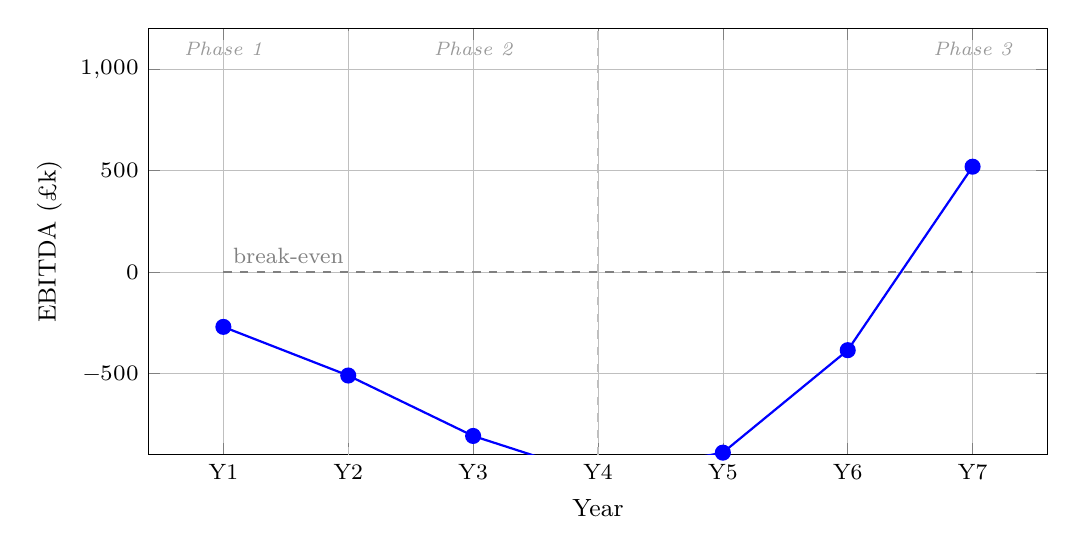
\begin{tikzpicture}
    \begin{axis}[
            width=13cm,
            height=7cm,
            xlabel={Year},
            symbolic x coords={Y1,Y2,Y3,Y4,Y5,Y6,Y7},
            xtick=data,
            grid=major,
            grid style={line width=.1pt, draw=gray!30},
            major grid style={line width=.2pt,draw=gray!50},
            legend style={
                font=\footnotesize,
                at={(0.02,0.98)},
                anchor=north west,
                legend cell align={left},
            },
            tick label style={font=\footnotesize},
            label style={font=\small},
        ylabel={EBITDA (\pounds k)},
        ymin=-900, ymax=1200,
    ]
    % Phase boundary markers (P1 ends Y2, P2 ends Y4)
    \draw[dashed,gray!50] (axis cs:Y2,-900) -- (axis cs:Y2,1200);
    \draw[dashed,gray!50] (axis cs:Y4,-900) -- (axis cs:Y4,1200);
    \node[anchor=north,font=\scriptsize\itshape,gray!80] at (axis cs:Y1,1180) {Phase 1};
    \node[anchor=north,font=\scriptsize\itshape,gray!80] at (axis cs:Y3,1180) {Phase 2};
    \node[anchor=north,font=\scriptsize\itshape,gray!80] at (axis cs:Y7,1180) {Phase 3};
    % EBITDA trajectory
    \addplot[thick,blue,mark=*,mark size=2.5pt,mark options={solid,fill=blue}] coordinates {(Y1,-270.0) (Y2,-509.4) (Y3,-806.8) (Y4,-1005.3) (Y5,-889.0) (Y6,-384.7) (Y7,518.5)};
    % Break-even reference line
    \draw[dashed,gray,thin] (axis cs:Y1,0) -- (axis cs:Y7,0);
    \node[anchor=west,font=\footnotesize,gray] at (axis cs:Y1,80) {break-even};
    \end{axis}
\end{tikzpicture}

\end{document}
